% Chapter Template

\chapter{Task Execution} % Main chapter title

\label{chapter:task_execution} % Change X to a consecutive number; for referencing this chapter elsewhere, use \ref{ChapterX}

\lhead{Chapter 7. \emph{Task Execution}} % Change X to a consecutive number; this is for the header on each page - perhaps a shortened title

This chapter shows how our system is able to execute tasks, and particularly joint actions. Section~\ref{sec:task_execution-intro} introduces the subject. Section~\ref{sec:task_execution-overview} describes our approach and the components that implement it. Section~\ref{sec:task_execution-action_executor} shows the main aspects of the Task Executor module, while section~\ref{sec:task_execution-collaborative_planners} introduces the framework we use to execute human-robot joint actions, the Collaborative Planners. Finally, section~\ref{sec:task_execution-handover} shows an example of a Collaborative Planner for human-robot handovers.


\section{Introduction}
\label{sec:task_execution-intro}
Acting in a human-crowded environment is a difficult problem. Even when acting independently, the robot needs: to ensure human safety, by taking others into account when planning and stopping if its actions could bring harm to them; to perform legible movements, so that its actions can be understood by humans (studied, for example, in~\cite{dragan2013legibility}); and to be robust, trying to complete its tasks even in front of unexpected conditions. 

These issues show us that humans should not be treated as simple obstacles by the robot, but need specialized reasoning and execution algorithms.

When performing a cooperative action with the human the robot needs to continuously monitor its partner, checking if he is involved in the task, stopping to wait for him, adapting its movements, and eventually abandoning the task, if the partner leaves. For example, if the robot is giving an object to a human, it will have to choose a position for its arm where the human can easily reach the object, change this position if the human is moving, and abandon the task if the human leaves the area.

\cite{bussy2012proactive} studied how to execute a transportation scenario jointly with a human partner, but the work is based more on haptic and control issues than actual reasoning, an area of the problem not deeply investigated.


\section{Overview}
\label{sec:task_execution-overview}

\subsection{Process Overview}

We have built a module to execute tasks, represented, as in the previous chapter, as \\ $(name, preconditions, target, postconditions)$, in a human-aware way. The focus of this module is not the planning or execution of the robot's motions, which are handled in external components, but the  execution of a \textit{task}, from start to finish. This problem presents several issues and steps:

\begin{itemize}
\item The robot needs to monitor if the task is actually achievable. Even though, if the task is part of a plan, our plan management algorithm, presented in section~\ref{sec:plan_management-plan_manager}, ensures that its preconditions are satisfied when it is executed, the task could still not be achievable. This problem may arise for different reasons. First, the robot is planning by using its knowledge of the state of the world, which may be faulty. For example, the robot might believe, when planning, that an object is on a table, and produce a plan where it will take it. If the location of the object is different, because it was moved without the robot knowing, the task might not be completed. Second, external events can happen that make a task unachievable, and the robot might not be able to detect or link these events to the task. For example, if a gush of wind throws the object to the floor, the robot might not immediately understand that this will prevent it, in the future, to take the object.
\item The system needs to interact with motion planners and executors to produce the range of movements needed by the robot to achieve its task.
\item The robot needs to constantly monitor its environment in order to ensure that the task is executed in a safe way. In particular, humans may move, while the robot is acting, in positions where they could be endanger by the robot's motions. To ensure human's safety, the robot needs to detect these situations and stop or pause its motions.
\item After a task is executed, the system needs to infer its effects, in order to update the knowledge on the state of the world. In general, a part of the postconditions of the actions could be observed by the robot. For example, if the robot has placed an object on a table, the robot could observe, and not only infer, its location. Since our perception can be faulty, if we do not integrate observation with inference, we might encounter situations where the robot is not able to observe the effects of its actions. For example, the robot has placed an object on the table, but the light conditions or the orientation of the object do not allow its recognition by the perception algorithms. To avoid this problem, the robot will update the position of the object using inference, in its mental model, and then refine it through observation, if it is able to see it.
\end{itemize}

We are particularly interested in the execution of human-robot joint actions. We have defined, in section~\ref{sec:overview-characteristics}, a joint action as a cooperative action between the two agents. As previously said, this kind of action requires additional mechanisms to allow the robot to cooperate with the human in a natural and efficient way. We developed a specific framework, which we called Collaborative Planners, to deal with this issue, which we present in section~\ref{sec:task_execution-collaborative_planners}.

\subsection{Architecture}

These ideas are represented in the following modules, as shown in figure~\ref{fig:task_execution:architecture}.
\begin{itemize}
	\item Task Executor. This module executes the robot's task in a robust, human-aware, and flexible way.
	\item Collaborative Planners. This set of planners are used to execute human-robot joint actions, allowing the robot to adapt its actions to the collaborators.
	\item Motion Planners and Executors. These planners, treated as external modules, are in charge of choosing trajectories for the robot, taking into account the environment and the present agents. We will not discuss this component, as it is outside the boundaries of this work. More details can be found in \cite{Sisbot2008,Mainprice2011,Pandey2010}.
\end{itemize}

We developed this layer with flexibility in mind. We can easily expand the system, by adding new actions, or switching motion planners and executors, without having an impact on the rest of the architecture.

\begin{figure}[h!]
	\centering
	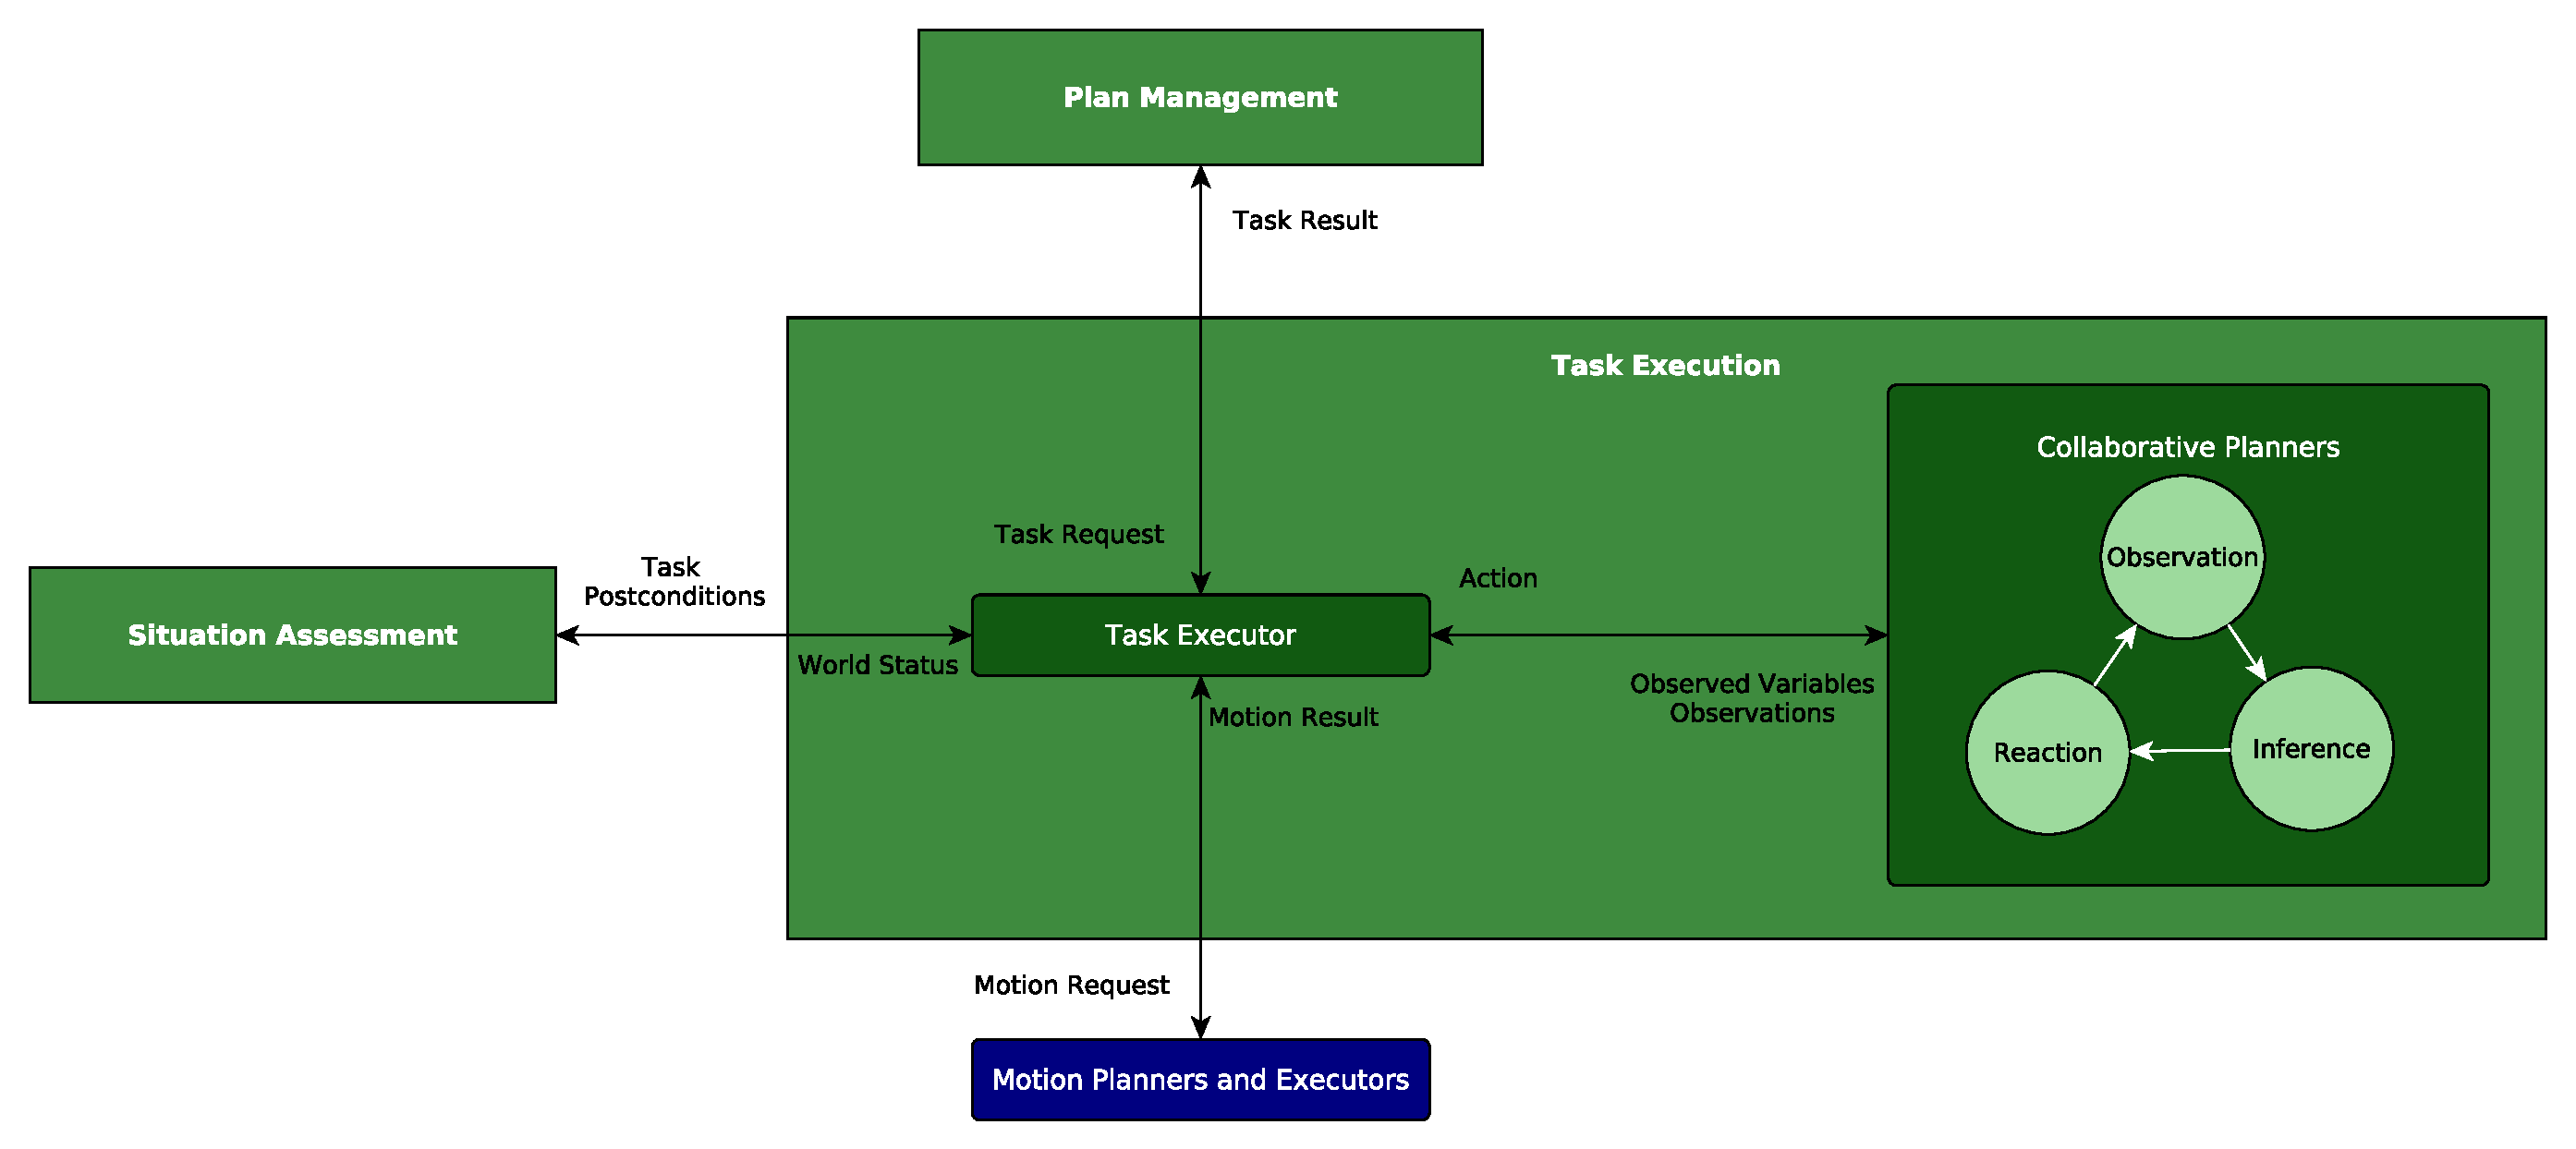
\includegraphics[clip,scale=0.38]{img/coworker/task_execution/architecture.pdf}
	\caption[The architecture of the Task Execution layer]{The architecture of the Task Execution  layer. Dark green rectangles represent modules, while light green rectangles layers. Blue rectangles represent external modules. Arrows represent messages exchanged between components, with the label detailing the message. The white ellipses, and their arrows, represent the process of the Collaborative Planners, explained in Section \ref{sec:task_execution-collaborative_planners}. While in this image we present the Collaborative Planners as a single unit, the system actually has a set of planners, and will choose, during the execution of a joint action, which one to use.}
	\label{fig:task_execution:architecture}
\end{figure}


Parts of this chapter where presented in~\cite{fioreiser2014}.

\section{Task Executor}
\label{sec:task_execution-action_executor}
The Task Executor handles task requests from the Plan Management layer. Following the ideas presented in section~\ref{sec:task_execution-overview}, the execution of a task is handled in several steps:
\begin{itemize}
\item Check Preconditions. The system can check if the preconditions of the task are valid by sending a query to the Situation Assessment layer. If the preconditions are not valid, the module returns an error.
\item Execute Task. The task is executed, by communicating with the Motion Planners and Executors and, if the current task is a joint action, with the Collaborative Planners.
\item Set Postconditions. The postconditions of the task are set in the Situation Assessment layer.
\end{itemize}

The execution of a task can fail, and in that case the world status is updated consequently. For example, if the robot is trying to pick an object, and the motion planner does not manage to compute a trajectory to reach it, the object will be considered as \textit{not reachable} by the robot in the current world status. When the Plan Management replans, the system could look for a plan where the robot changes position and tries again the pick, or even asks another agent to give him the object.

Tasks can be paused and resumed. We set a number of safety rules, where the robot will pause executing a motion if a human, or one of his body parts, is too close to the robot's grippers or arms.

The robot is also able to show some social clues during an action, for example by moving its head toward the tasks' $target$. 

\section{Collaborative Planners} 
\label{sec:task_execution-collaborative_planners}
When executing joint actions with humans, the robot needs to continuously observe its partner and react appropriately. The robot's action should be based on different aspects. First of all, the robot should act differently depending on the current status and level of advancement of the task. Second, the robot should consider the status of the world, in order to take appropriate actions. Then, as we said, the robot should observe its partner's behavior, which can give different information. Of course, the robot should coordinate with the human's movements. For example, if the two agents are performing an handover, and the human extends his hand, the robot should extend its arm to bring the object in a reachable position.

Observing the human's activities can give us more subtle information, that represent how much he is engaged in the task. For example, in the case of the handover, if the human is oriented toward the robot and extending his hand, we can assume that he is currently engaged and cooperating. If, instead, the human is looking in another direction, or moving away, we can infer that he is currently doing something else, and perhaps has even abandoned the task.

To reason on all these variables and produce an appropriate reaction, we introduced a special framework to manage cooperative actions, called the Collaborative Planners, based on hierarchical Mixed Observability Markov Decision Processes (MOMDP). A MOMDP can be modeled as a tuple $(S_h,S_o,A,T,R,\Omega,O,\gamma)$, where $S_h$ is the hidden state, $S_o$ is the observed state, $A$ is the set of actions, $T$ is the transition function, $R$ is the reward function, $\Omega$ is the observation function, $O$ is the set of observations, and $\gamma$ is a discount factor. More details about Markov Models are provided in appendix~\ref{appendix-methods}.

Using n MMODP we can model observed variables, like the task and world status, and hidden variables, like the engagement level of the human, which we can infer from observations. Using a hierarchy of models, as explained in \cite{pineau2001hierarchical}, we can represent complex scenarios and tasks with smaller, simpler models, that can be solved more easily, and expand them by adding more actions and complex behaviors as we see fit.

For each joint actions, we will introduce a new Collaborative Planner. When the system is executing a joint action between the robot and a human, the Task Executor will contact the related Collaborative Planner.  The Task Executor will send requests containing the observations and observed variables, used to update the MMODPs, and the planner will return a sub-action to execute. To maintain this model generic the Collaborative Planners will output high-level actions, which the Task Executor will adapt to the current situation. This process will continue until the joint action is achieved, the planner chooses to abandon the task, or there is a failure.

We provide a \textit{basic framework} that we use to implement Collaborative Planners, that can be adapted to the specific task. While it is not obligatory to implement a Collaborative Planner following these ideas, we believe that they offer a good basis for cooperative tasks:

\begin{itemize}
	\item $S_h=\{human\_commitment\}$
		\begin{itemize}
			\item $values(human\_commitment)=\{engaged,not\_engaged,not\_interested\}$.
		\end{itemize}  

		The human commitment to the task can be modeled as a hidden variable.  A user can be engaged in the task, meaning that he is actively participating; not engaged, meaning that he is currently not participating, but we expect that he will resume the task (imagine, for example, a user receiving a phone call while executing a joint task); or not interested, meaning that he has abandoned the task. 

		Modeling the human commitment is very important, since the robot should choose its action based on this variable, and of course on other task related variables. For example, if the user is not currently engaged in the task, the robot might choose to wait for him, or ask him if he has a problem. If he has abandoned the task, the robot might look for another plan, or ask the help of another human. If he is committed, the robot could proceed to accomplish the task, as long as the world state allows it.

	\item $S_o:\{task\_advancement\}$.
		\begin{itemize}
			\item $values(task\_advancement)=\{not\_started,started,completed\}$.
		\end{itemize}

		The status of advancement of the task can provide useful information to help the robot  choose its actions. A simple way to represent it is considering just an initial state, where the agents have decided to execute a cooperative task, but have not started executing it yet; a middle state, where the agents are working to complete the task; and a final state, where the task is completed. Different tasks could further refine this variable.
	\item $A:\{continue,wait,abandon,engage\}$.

		When building an action set, the developer should consider how much control the MOMDP should have over the robot's actions. In our implementations, we chose to plan generic high level actions, that will be adapted by the Task Executor. This strategy allows us to simplify the state space of the MOMDP. In a basic Collaborative Planner, the robot is able to: continue its task, meaning that it will take the next logical action depending on the current state, maintained by the Task Executor; wait for the user, if the robot detects that he is momentarily not engaged in the task; abandon, if the user is not interested anymore in executing the task; engage, to communicate with the user, for example by giving him a warning.

	\item $T$, $R$ and $O$ are, of course, completely dependent on the joint task.
	\item $\Omega$ is dependent on the current application. Some typical observations are related to spatial relationships between the user and the robot (e.g. the user is more likely to be interested in the task if he is close to the robot and oriented toward him), or particular poses of the user (e.g. the user is ready to receive an object if he has extended its arm toward the robot).

\end{itemize}

Our idea is similar to the work of \cite{ferrari2015hierarchical}. The authors propose a framework based on hierarchical POMDPs for cooperative tasks, with a three layer structure. This framework was applied to an escort application, where the robot had to guide a user to his location in a human-aware way, adapting to his behaviors. In this application, the commitment of the user is estimated by reasoning on how much the human is focused on the robot, and on their distance.
We implemented a similar application, for a robot guide, using our Collaborative Planners, which we will show in part~\ref{part:case_study}. The main difference between our framework and the one developed by the authors is that they chose to give a much stronger decision power to the POMDP, while in our system planning is actually split among several units, and the Task Execution module has a big role in adapting the actions of the Collaborative Planners. We also do note use a precise hierarchical framework, leaving to the single Collaborative Planners the choice on how many layers of task to use.

We will show, in the next section, an example of collaborative planner which develops this basic framework.

\section{Collaborative Planner for Handover}
\label{sec:task_execution-handover}
The handover collaborative planner has the goal to handle both human-robot and robot-human handovers in a human-aware way. We will show parts of this model now, avoiding the observation and transition function, as they are extensive and do not provide particular help in understanding this example.

\begin{itemize}
	\item $S_h:\{human\_commitment\}$.
		The hidden variable, and its values, follow the basic framework presented in the previous section.
	\item $S_o:\{task\_advancement\, timer, human\_distance\}$.
		\begin{itemize}
			\item $value(task\_advancement)=\{not\_started,started,touching,completed\}$.
			\item $values(timer)=\{not\_expired,expired\}$.
			\item $values(human\_distance)=\{close, far, out\_of\_range\}$.
		\end{itemize}

		The task advancement is represented in a similar way as the basic framework. We add the $touching$ value to this variable, representing the fact that the gripper of the robot has detected some pressure (e.g. the human has placed an object in it, if the handover is human-robot, or he has grabbed the object kept in the gripper, if the handover is robot-human).
		 We add a timer variable, which is started and controller by the Task Executor when the robot is waiting for the user. When the timer expires in the Task Executor, this variable will be set accordingly, and the robot can perform specific actions (e.g. ask the user if he still wants to perform the task).
		 We also consider the human distance from the robot, classifying it as $close$ to the robot, $far$ from the robot, and $out\_of\_range$ if the human is not visible. 
	\item $A:\{continue,wait,abandon,engage\}$.

		The actions follow the basic framework. The $continue$ action is chosen when the user is $engaged$. The Task Executor will react differently to this action, dependently on the current $task\_advancement$. If $task\_advancement \neq touching$ then the robot will extend (or keep extended) the arm toward the user. If $task\_advancement=touching$ the robot will release the object, or grab it from the human's hand, depending on the kind of handover.

		The $wait$ action is chosen when the user is $not\_engaged$. In this case the robot will retract its hand to an intermediate position. The Task Executor will start a timer.

		The $abandon$ action is chosen when the user is $not\_interested$ or the task is $completed$.

		Finally, the $engage$ action is chosen when the $timer$ is $expired$. In this case the robot will ask the human if he still wants to perform the handover.
	\item $O:\{human\_arm,human\_orientation,human\_distance\_variation\}$.
		\begin{itemize}
			\item $values(human\_arm)=\{approaching,retracting,still,unknown\}$.
			\item $values(human\_orientation)=\{toward\_robot,other,unknown\}$.
			\item $values(human\_distance\_variation)=\{decreasing,increasing,still,unknown\}$.
		\end{itemize}

		We present several human observations, used to estimate his engagement. In general, we consider that the human is more likely to be $engaged$ when he is approaching the robot, he is turned toward it, and his arm is extending. If the human is turned away, or even leaving, it is more likely that he is currently $not\_engaged$ or even $not\_interested$. Finally, if the human is $out\_of\_range$, his observations will be $unknown$, since the robot does not know his location.

	\item  $R$: the robot is rewarded for completing the task, performing the handover, and for executing desirable behaviors, like waiting for a user if we detect that he is not engaged, and abandoning the task if he is no longer interested in the joint action. 
\end{itemize}

An example of handover using this Collaborative Planner is shown in figure~\ref{fig:task_execution-handover}.

\begin{figure}[h!]
	\centering
	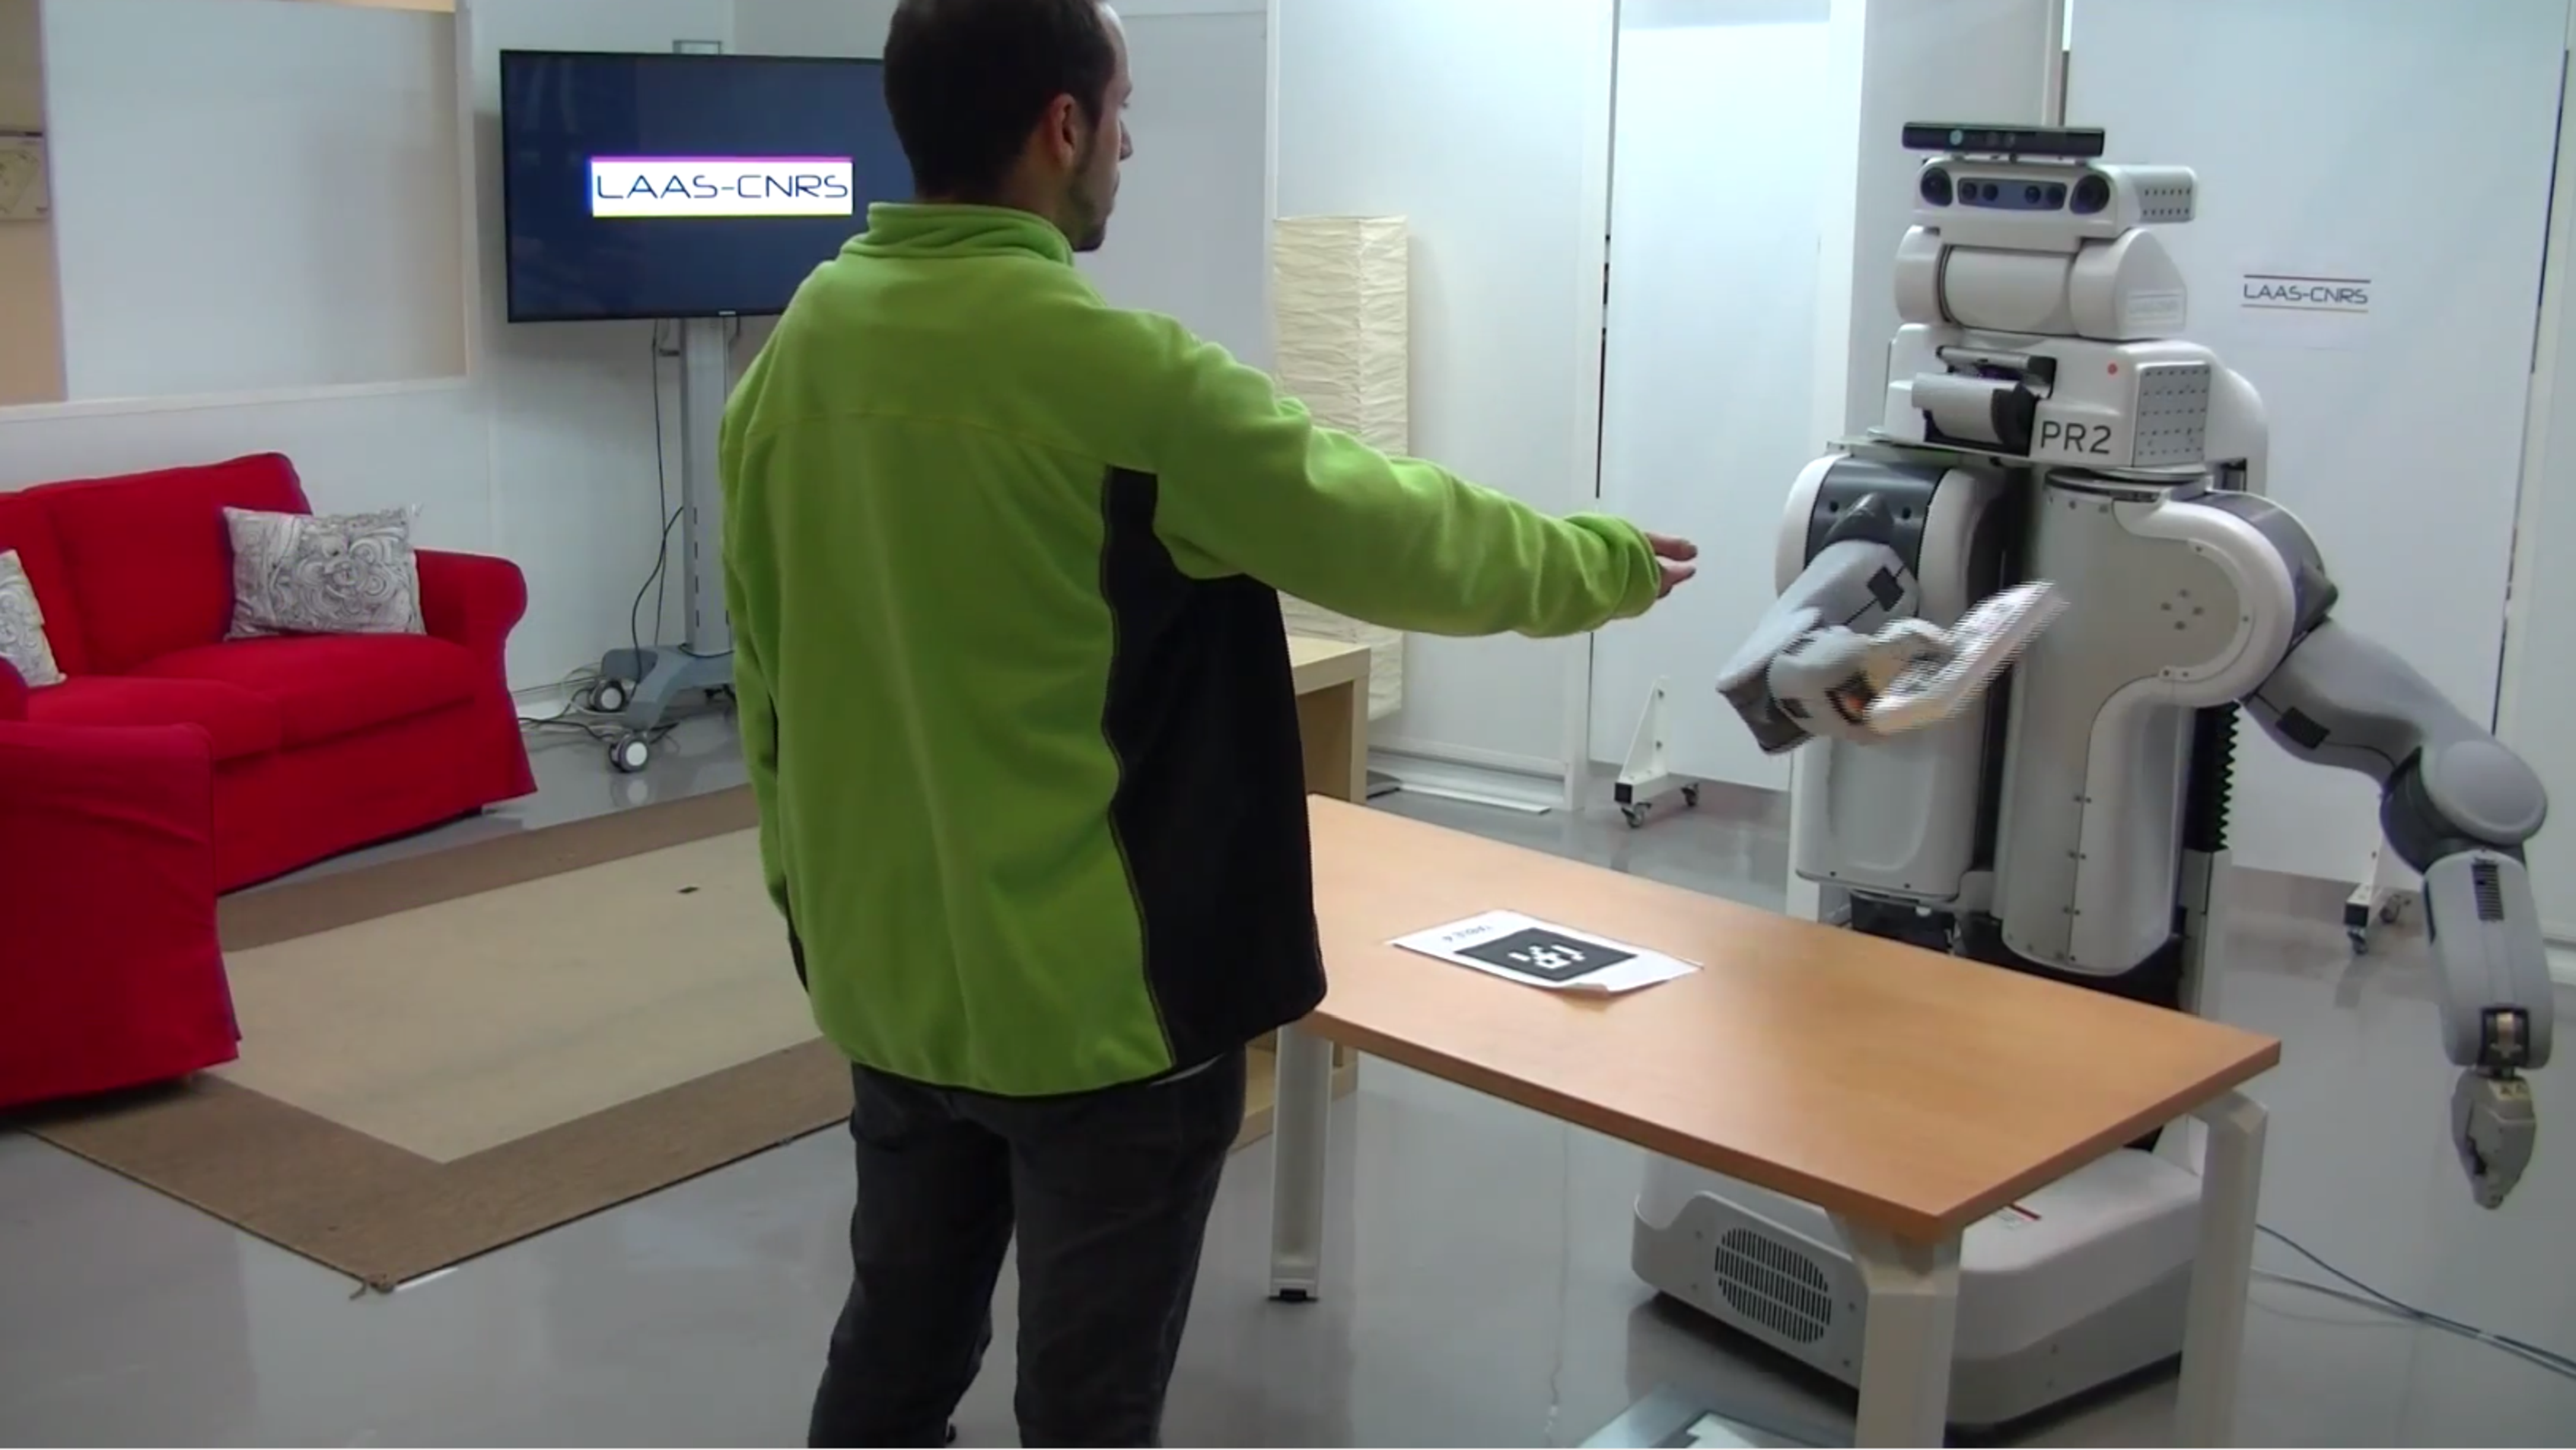
\includegraphics[scale=0.3]{img/coworker/task_execution/handover.pdf}
	\caption[Handover]{A robot-human handover}
	\label{fig:task_execution-handover}
\end{figure}
